\chapter{Specifikacija programske potpore}
		
	\section{Funkcionalni zahtjevi}
			
			
			\noindent \textbf{Dionici:}
			
			\begin{packed_enum}
				
				\item Skladištar
				\item Šef skladišta			
				\item Direktor
				\item Razvojni tim
				
			\end{packed_enum}
			
			\noindent \textbf{Aktori i njihovi funkcionalni zahtjevi:}
			
			
			\begin{packed_enum}
				\item	\underbar{Skladištar (inicijator) može:}
					
					\begin{packed_enum}
						\item Skenirati artikle za inventuru
						\item Pristupiti povijesti svih svojih unosa
						\item Dojaviti šefu skladišta da artikla nema na skladištu
						\item Odjaviti se
					\end{packed_enum}

				\item  \underbar{Šef skladišta (inicijator) može:}
					
					\begin{packed_enum}
						\item Skenirati artikle za inventuru
							\begin{packed_enum}
								\item Kao kontrolor
								\item Kao izvršitelj inventure
							\end{packed_enum}
						\item Vidjeti sve artikle na skladištu u kojem je nadležan
						\item Pristupiti povijesti svih svojih unosa
						\item Primati obavijesti o nedostatku pojedinog artikla koje dojavi skladištar
							\begin{packed_enum}
								\item Proslijediti tu obavijest direktoru
							\end{packed_enum}
						\item Odjaviti se
					\end{packed_enum}

				\item  \underbar{Direktor (inicijator) može:}
				
				\begin{packed_enum}
					\item Skenirati artikle za inventuru
					\item Vidjeti povijest svih svojih unosa
					\item Vidjeti stanje artikala na svim skladištima
					\item Vidjeti statistiku pogrešaka svakog skladištara
					\item Izabrati skladišta koje želi provjeriti
						\begin{packed_enum}
							\item Izabrati inventure na odabranom skladištu
							\item Pregledati sve skenirane artikle u toj inventuri
						\end{packed_enum}
					\item Dodati novo skladište
					\item Urediti stablo artikala
						\begin{packed_enum}
							\item Dodati artikl
							\item Ukloniti Artikl
							\item Dodati kategoriju
							\item Ukloniti kategoriju
						\end{packed_enum}
					\item Pristupiti svim obavijestima
					\begin{packed_enum}
						\item Razriješiti obavijesti
					\end{packed_enum}
					\item Odjaviti se
				\end{packed_enum}
			
			
			\item	\underbar{Baza podataka (sudionik)}
				\begin{packed_enum}
					\item Pohranjivati sve podatke o korisnicima i njihovim ovlastima
					\item Pohranjivati sve podatke o inventurama, skladištima, obavijestima i artiklima
				\end{packed_enum}
			\end{packed_enum}
			
			\eject 
			
			
				
			\subsection{Obrasci uporabe}
				
				
				\subsubsection{Opis obrazaca uporabe}
					
					\noindent \underbar{\textbf{UC1 - Registracija}}
					\begin{packed_item}
	
						\item \textbf{Glavni sudionik: }Korisnik
						\item  \textbf{Cilj:} Stvoriti korisnički račun za pristup sustavu
						\item  \textbf{Sudionici:} Baza podataka
						\item  \textbf{Preduvjet:} -
						\item  \textbf{Opis osnovnog tijeka:}
						
						\item[] \begin{packed_enum}
	
							\item Korisnik odabire opciju za registraciju
							\item Korisnik unosi potrebne korisničke podatke te bira jednu od ponuđenih uloga
							\item Podaci se spremaju u bazu podataka
														
						\end{packed_enum}
						
						\item  \textbf{Opis mogućih odstupanja:}
						
						\item[] \begin{packed_item}
	
							\item[2.a] Odabir email adrese koja se već koristi, unos podataka u nedozvoljenom formatu, ne popunjavanje svih potrebnih podataka 
							\item[] \begin{packed_enum}
								
								\item Sustav obavještava korisnika o neuspjelom upisu i vraća ga na stranicu za prijavu
								\item Korisnik mijenja potrebne podatke te završava unos ili odustaje od registracije
								
							\end{packed_enum}
						\end{packed_item}
					\end{packed_item}
				

					\noindent \underbar{\textbf{UC2 - Prijava u sustav}}
					\begin{packed_item}
	
						\item \textbf{Glavni sudionik: }Skladištar, šef skladišta, direktor
						\item  \textbf{Cilj:} Prijaviti se u sustav i dobiti pristup korisničkom sučelju
						\item  \textbf{Sudionici:} Baza podataka
						\item  \textbf{Preduvjet:} Registracija
						\item  \textbf{Opis osnovnog tijeka:}
						
						\item[] \begin{packed_enum}
	
							\item Korisnik unosi email adresu i lozinku
							\item Uspoređuje se korisnikov unos s podacima u bazi podataka 
							\item Prikazuje se početni zaslon aplikacije
							
						\end{packed_enum}
						
						\item  \textbf{Opis mogućih odstupanja:}
						
						\item[] \begin{packed_item}
	
							\item[2.a] Neispravna email adresa  ili lozinka
							\item[] \begin{packed_enum}
								
								\item Sustav obavještava korisnika o neuspjelom upisu i vraća ga na stranicu za registraciju\\
								
							\end{packed_enum}
						\end{packed_item}
					\end{packed_item}
				
		
					\noindent \underbar{\textbf{UC3 - Odjava iz sustava}}
					\begin{packed_item}
	
						\item \textbf{Glavni sudionik: }Skladištar, šef skladišta, direktor
						\item  \textbf{Cilj:} Odjaviti se iz sustava
						\item  \textbf{Sudionici:} Baza podataka
						\item  \textbf{Preduvjet:} Korisnik je prijavljen u sustav
						\item  \textbf{Opis osnovnog tijeka:}
						
						\item[] \begin{packed_enum}
	
							\item Korisnik odabire opciju "Odjava" s ikonom mobilnog uređaja i strelice u gornjem desnom kutu
							\item Prikazuje se stranica za registraciju 
														
						\end{packed_enum}
					\end{packed_item}	
					
					\noindent \underbar{\textbf{UC4 - Skeniranje artikla}}
					\begin{packed_item}
	
						\item \textbf{Glavni sudionik: }Skladištar, šef skladišta, direktor
						\item  \textbf{Cilj:} Skenirati artikl
						\item  \textbf{Sudionici:} Baza podataka
						\item  \textbf{Preduvjet:} Korisnik je prijavljen u sustav i odabrao je koji artikl želi skenirati
						\item  \textbf{Opis osnovnog tijeka:}
						
						\item[] \begin{packed_enum}
							
							\item Korisnik postavlja mobilni uređaj iznad bar ili QR koda koji želi skenirati
							\item Korisnik pritiskom na ikonu QR koda (sredina, dolje) skenira kod artikla
							\item Prikazuje se pop-up window s informacijama o skeniranom artiklu
							\item Korisnik u pop-up window-u odabire mogućnost povećanja ili smanjenja broja takvih artikala na skladištu pritiskom na ikone "-" i "+", odbacivanja trenutno skeniranog proizvoda bez spremanja u bazu pritiskom na opciju "Odbaci", spremanje artikla u bazu pritiskom na opciju "Spremi" te izlaska iz pop-up window-a pritiskom na opciju "Završi"
							
						\end{packed_enum}
						
						\item  \textbf{Opis mogućih odstupanja:}
						
						\item[] \begin{packed_item}
	
							\item[2.a] Skenirani artikl ne postoji u bazi podataka
							\item[] \begin{packed_enum}
								
								\item Sustav obavještava korisnika o neuspjelom pokušaju skeniranja uz poruku "Skenirani artikl ne postoji u bazi podataka" te ga vraća na početni zaslon za skeniranje artikala								
							\end{packed_enum}
						
							\item[2.b] Skenirani artikl nije onaj odabrani
							\item[] \begin{packed_enum}
								\item Sustav obavještava korisnika o neuspjelom pokušaju skeniranja uz poruku "Skenirani artikl nije onaj odabrani" te ga vraća na početni zaslon za skeniranje artikala\\  
							\end{packed_enum}
						\end{packed_item}
					\end{packed_item}
				
					\noindent \underbar{\textbf{UC5 - Završetak skeniranja artikla}}
					\begin{packed_item}
						\item \textbf{Glavni sudionik: }Skladištar, šef skladišta, direktor
						\item  \textbf{Cilj:} Završiti sa skeniranjem odabranog artikla
						\item  \textbf{Sudionici:} Baza podataka
						\item  \textbf{Preduvjet:} Korisnik je prijavljen u sustav i odabrao je artikl koji želi skenirati
						\item  \textbf{Opis osnovnog tijeka:}
						\item[] \begin{packed_enum}
							\item Korisnik na početnom zaslonu pritišće gumb "Završi"
							\item Korisnik potvrđuje da želi završiti sa skeniranjem odabranog artikla
						\end{packed_enum}
					\end{packed_item}
					
					
					\noindent \underbar{\textbf{UC6 - Pregled povijesti inventura}}
					\begin{packed_item}
	
						\item \textbf{Glavni sudionik: }Skladištar, šef skladišta
						\item  \textbf{Cilj:} Pregled svih unosa artikala po inventurama
						\item  \textbf{Sudionici:} Baza podataka
						\item  \textbf{Preduvjet:} Korisnik je prijavljen u sustav
						\item  \textbf{Opis osnovnog tijeka:}
						
						\item[] \begin{packed_enum}
	
							\item Korisnik pritišće ikonu liste u donjem lijevom kutu početnog zaslona
							\item Prikazuje se popis inventura 
							\item Korisnik bira inventuru
							\item Prikazuje se popis skeniranih artikala 
														
						\end{packed_enum}
					\end{packed_item}
					
					
					\noindent \underbar{\textbf{UC7 - Pregled povijesti inventura}}
					\begin{packed_item}
	
						\item \textbf{Glavni sudionik: }Direktor
						\item  \textbf{Cilj:} Pregled svih unosa artikala po inventurama u svim skladištima 
						\item  \textbf{Sudionici:} Baza podataka
						\item  \textbf{Preduvjet:} Korisnik je prijavljen u sustav
						\item  \textbf{Opis osnovnog tijeka:}
						
						\item[] \begin{packed_enum}
	
							\item Korisnik pritišće ikonu liste u donjem lijevom kutu početnog zaslona
							\item Prikazuje se popis svih skladišta
							\item Korisnik bira skladište
							\item Prikazuje se popis inventura 
							\item Korisnik bira inventuru
							\item Prikazuje se popis skeniranih artikala \\
							\newline
							\newline
																				
						\end{packed_enum}
					\end{packed_item}
					
					
					\noindent \underbar{\textbf{UC8 - Dojava da određenog artikla nema na skladištu}}
					\begin{packed_item}
	
						\item \textbf{Glavni sudionik: }Skladištar, šef skladišta
						\item  \textbf{Cilj:} Dojaviti nadređenima da određenog artikla nema na skladištu
						\item  \textbf{Sudionici:} Baza podataka
						\item  \textbf{Preduvjet:} Korisnik je prijavljen u sustav
						\item  \textbf{Opis osnovnog tijeka:}
						
						\item[] \begin{packed_enum}
	
							\item Korisnik odabire opciju "Nema artikla"
							\item Korisnik odabire naziv artikla
							\item Korisnik odabire opciju "Dojavi"
														
						\end{packed_enum}
					\end{packed_item}
					
					
					\noindent \underbar{\textbf{UC9 - Pregled obavijesti}}
					\begin{packed_item}
	
						\item \textbf{Glavni sudionik: }Šef skladišta
						\item  \textbf{Cilj:} Pregled obavijesti koje su poslali skladištari
						\item  \textbf{Sudionici:} Baza podataka
						\item  \textbf{Preduvjet:} Korisnik je prijavljen u sustav
						\item  \textbf{Opis osnovnog tijeka:}
						
						\item[] \begin{packed_enum}
	
							\item Korisnik odabire opciju s ikonom pošte 
							\item Prikazuje se stranica s obavijestima o artiklima kojih nema na skladištu
							\item Korisnik odabire opciju "Šalji direktoru" ako to smatra opravdanim
							\item Odabrana obavijest se šalje direktoru
														
						\end{packed_enum}
					\end{packed_item}
					
					
					\noindent \underbar{\textbf{UC10 - Pregled obavijesti}}
					\begin{packed_item}
	
						\item \textbf{Glavni sudionik: }Direktor
						\item  \textbf{Cilj:} Pregled obavijesti koje su poslali šefovi skladišta
						\item  \textbf{Sudionici:} Baza podataka
						\item  \textbf{Preduvjet:} Korisnik je prijavljen u sustav
						\item  \textbf{Opis osnovnog tijeka:}
						
						\item[] \begin{packed_enum}
	
							\item Korisnik odabire opciju s ikonom pošte 
							\item Prikazuje se stranica s obavijestima o artiklima kojih nema na skladištu i o pogreškama skladištara 
							\item Korisnik odabire kvačicu ako želi određenu obavijest označiti kao riješenu, križić ako ju želi označiti kao odbačenu, ili opcije "Razriješi sve" i "Odbaci sve"\\
							\newline
														
						\end{packed_enum}
					\end{packed_item}
					
					
					\noindent \underbar{\textbf{UC11 - Pregled svih artikala na skladištu}}
					\begin{packed_item}
	
						\item \textbf{Glavni sudionik: }Šef skladišta
						\item  \textbf{Cilj:} Pregled broj svih artikala na skladištu
						\item  \textbf{Sudionici:} Baza podataka
						\item  \textbf{Preduvjet:} Korisnik je prijavljen u sustav
						\item  \textbf{Opis osnovnog tijeka:}
						
						\item[] \begin{packed_enum}
	
							\item Korisnik odabire opciju s ikonom kuće
							\item Prikazuje se popis artikala u skladištu temeljem zadnje odrađene inventure i njihova količina 
																					
						\end{packed_enum}
					\end{packed_item}
					
					
					\noindent \underbar{\textbf{UC12 - Pregled svih skladišta kompanije}}
					\begin{packed_item}
	
						\item \textbf{Glavni sudionik: }Direktor
						\item  \textbf{Cilj:} Pregled svih skladišta kompanije te artikala i skladištara u njima 
						\item  \textbf{Sudionici:} Baza podataka
						\item  \textbf{Preduvjet:} Korisnik je prijavljen u sustav
						\item  \textbf{Opis osnovnog tijeka:}
						
						\item[] \begin{packed_enum}
							
							\item Korisnik odabire opciju s ikonom kuće
							\item Prikazuje se popis skladišta
							\item Korisnik bira skladište
							\item Prikazuje se popis artikala i skladištara u odabranom skladištu 
							\item Korisnik odabire opciju "Artikl"
							\item Prikazuje se popis artikala u odabranom skladištu 
							\item Korisnik odabire opciju "Skladištar"
							\item Prikazuje se popis skladištara i njihova statistika pogreške u odabranom skladištu 
																												
						\end{packed_enum}
					\end{packed_item}
					
					
					\noindent \underbar{\textbf{UC13 - Dodavanje skladišta}}
					\begin{packed_item}
	
						\item \textbf{Glavni sudionik: }Direktor
						\item  \textbf{Cilj:} Dodati novo skladišta
						\item  \textbf{Sudionici:} Baza podataka
						\item  \textbf{Preduvjet:} Korisnik je prijavljen u sustav
						\item  \textbf{Opis osnovnog tijeka:}
						
						\item[] \begin{packed_enum}
	
							\item Korisnik odabire opciju "+" na stranici s popisom skladišta
							\item Prikazuje se stranica za unos novog skladišta
							\item Korisnik unosi novo skladište
							\item Korisnik izabire drugog korisnika s oznakom "Šef skladišta" za odabranu lokaciju
							\item Novo skladište se sprema u bazu podataka
																												
						\end{packed_enum}
					\end{packed_item}
				
					\noindent \underbar{\textbf{UC14 - Brisanje skladišta}}
					\begin{packed_item}
						
						\item \textbf{Glavni sudionik: }Direktor
						\item  \textbf{Cilj:} Obrisati skladište
						\item  \textbf{Sudionici:} Baza podataka
						\item  \textbf{Preduvjet:} Korisnik je prijavljen u sustav i skladište postoji
						\item  \textbf{Opis osnovnog tijeka:}
						
						\item[] \begin{packed_enum}
							\item Korisnik odabire skladište koje želi obrisati
							\item Korisnik pritiskom na ikonu kante za smeće briše odabrano skladište
						\end{packed_enum}
						
						
					\end{packed_item}
					
					
					\noindent \underbar{\textbf{UC15 - Dodavanje artikla}}
					\begin{packed_item}
	
						\item \textbf{Glavni sudionik: }Direktor
						\item  \textbf{Cilj:} Dodati novi artikl ili kategoriju proizvoda 
						\item  \textbf{Sudionici:} Baza podataka
						\item  \textbf{Preduvjet:} Korisnik je prijavljen u sustav
						\item  \textbf{Opis osnovnog tijeka:}
						
						\item[] \begin{packed_enum}
	
							\item Korisnik odabire opciju "+" na stranici s popisom artikala
							\item Prikazuje se stranica za unos novog artikla 
							\item Korisnik unosi novi artikl ili kategoriju
							\item Promjene se spremaju u bazu podataka
																					
						\end{packed_enum}
					\end{packed_item}
					
					\noindent \underbar{\textbf{UC16 - Preraspodjela artikla}}
					\begin{packed_item}
						\item \textbf{Glavni sudionik: }Direktor
						\item  \textbf{Cilj:} Preraspodijeliti postojeći artikl 
						\item  \textbf{Sudionici:} Baza podataka
						\item  \textbf{Preduvjet:} Korisnik je prijavljen u sustav i artikl postoji u sustavu
						\item  \textbf{Opis osnovnog tijeka:}
						
						\item[] \begin{packed_enum}
							\item Korisnik odabire koji proizvod želi preraspodijeliti
							\item Otvara se pop-up window sa mogućnosti odabira nove kategorije
							\item Korisnik odabire u novu kategoriju
							\item Korisnik potvrđuje novu kategoriju
							\item Proizvod ili kategorija proizvoda se preraspodijeli u novu kategoriju
							\newline
						\end{packed_enum}
					
						
					\end{packed_item}
				
					\noindent \underbar{\textbf{UC17 - Brisanje artikla}}
					\begin{packed_item}
						\item \textbf{Glavni sudionik: }Direktor
						\item  \textbf{Cilj:} Obrisati postojeći artikl ili kategoriju proizvoda 
						\item  \textbf{Sudionici:} Baza podataka
						\item  \textbf{Preduvjet:} Korisnik je prijavljen u sustav i artikl postoji u sustavu
						\item  \textbf{Opis osnovnog tijeka:}
						
						\item[] \begin{packed_enum}
							\item Korisnik odabire koji proizvod ili kategoriju proizvoda želi obrisati
							\item Otvara se pop-up window sa upozorenjem
							\item Korisnik potvrđuje da želi obrisati proizvod
						\end{packed_enum}
					\item  \textbf{Opis mogućih odstupanja:} 
					\item[] \begin{packed_item}
						
						\item[2.a] Čvor kategorije proizvoda koji se želi obrisati ima djecu
						\item[] \begin{packed_enum}
							
							\item Sustav obavještava korisnika o pogrešci i ne dozvoljava brisanje kategorije proizvoda
							
						\end{packed_enum}
					\end{packed_item}
					
					\end{packed_item}
				
					\noindent \underbar{\textbf{UC18 - Završetak inventure}}
					\begin{packed_item}
						\item \textbf{Glavni sudionik: }Direktor
						\item  \textbf{Cilj:} Završiti inventuru i započeti sljedeću
						\item  \textbf{Sudionici:} Baza podataka
						\item  \textbf{Preduvjet:} Korisnik je prijavljen u sustav i inventura traje
						\item  \textbf{Opis osnovnog tijeka:}
						
						\item[] \begin{packed_enum}
							\item Korisnik na početnom zaslonu odabire gumb "završi inventuru"
							\item Korisnik potvrđuje da želi završiti inventuru
							\item Trenutna inventura završava te se svi njezini unosi šalju u bazu podataka
							\item Automatski počinje nova inventura
						\end{packed_enum}
					\end{packed_item}

				\subsubsection{Dijagrami obrazaca uporabe}
					
					\begin{figure}[H]
						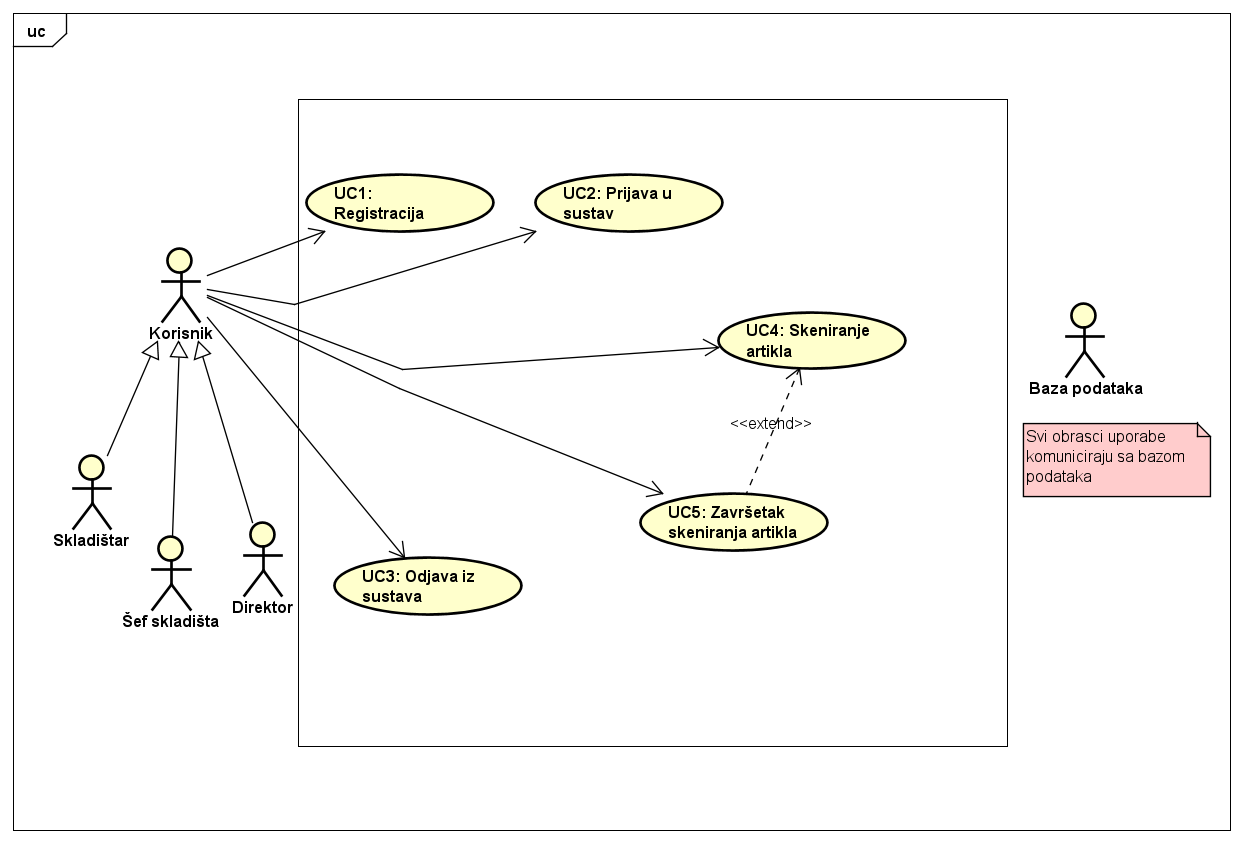
\includegraphics[scale=0.5]{slike/uc1.png}
						\caption{Dijagram obrasca uporabe, zajedničke funkcionalnost svih korisnika}
						
					\end{figure}
				
					\begin{figure}[H]
						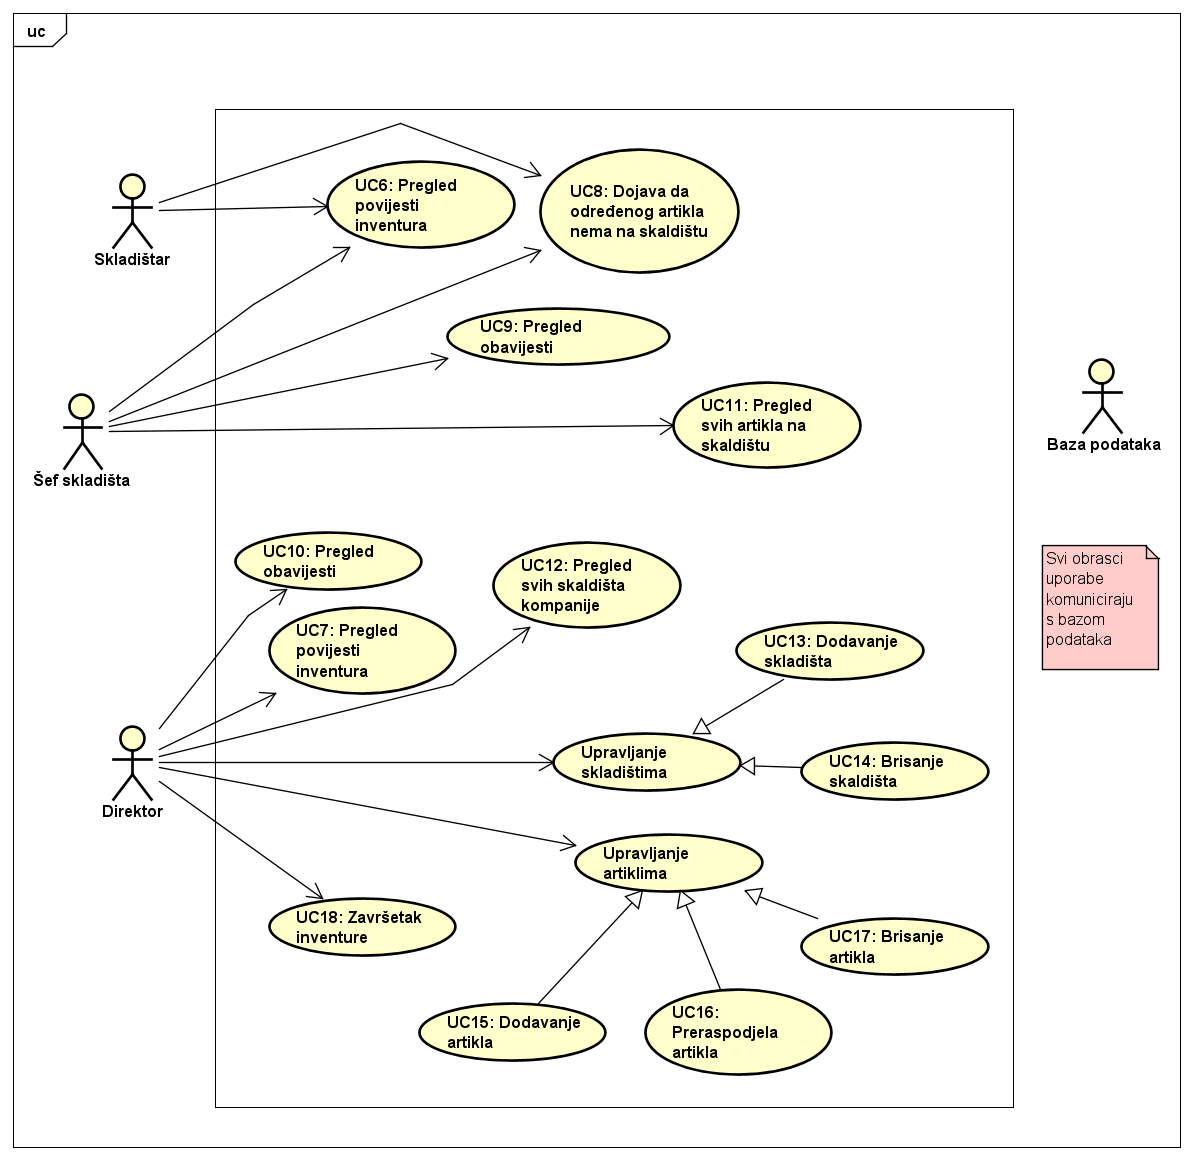
\includegraphics[scale=0.5]{slike/uc2.png}
						\caption{Dijagram obrasca uporabe, zasebne funkcionalnost skladištara, šefa skladišta i direktora}
					\end{figure}
				
			\subsection{Sekvencijski dijagrami}
				
				\textbf{Obrazac uporabe UC4 - Skeniranje artikla}
				
				Korisnik detekcijom koda šalje zahtjev mobilnoj aplikaciji za prikaz informacija o artiklu kako bi mogao uređivati broj tog artikla na skladištu. Ukoliko u bazi podataka ne postoji artikl sa odgovarajućim kodom mobilna aplikacija korisniku na zaslon ispiše odgovarajuću obavijest. Inače ako skenirani artikl nije onaj koji se trenutno skenira mobilna aplikacija također korisniku ispiše odgovarajuću obavijest. Ako u bazi podataka postoji artikl sa odgovarajućim kodom i ako je taj artikl onaj koji se trenutno skenira, mobilna aplikacija dohvaća podatake o artiklu i u obliku pop-up prozora prikazuje te informacije. Na zaslonu s informacijama o skeniranom proizvodu korisniku se nudi opcija da poveća ili smanji broj takvih artikala u skladištu, da odbaci trenutno očitanje bez spremanja u bazu ili da trenutno očitanje odmah pohrani u bazu (bez čekanja da istekne 5 sekundi). Promjenom broja očitanih artikala resetira se brojač 5 sekundi. Istekom vremena brojača zapis se automatski pohranjuje u bazu.
				
			\begin{figure}[H]
				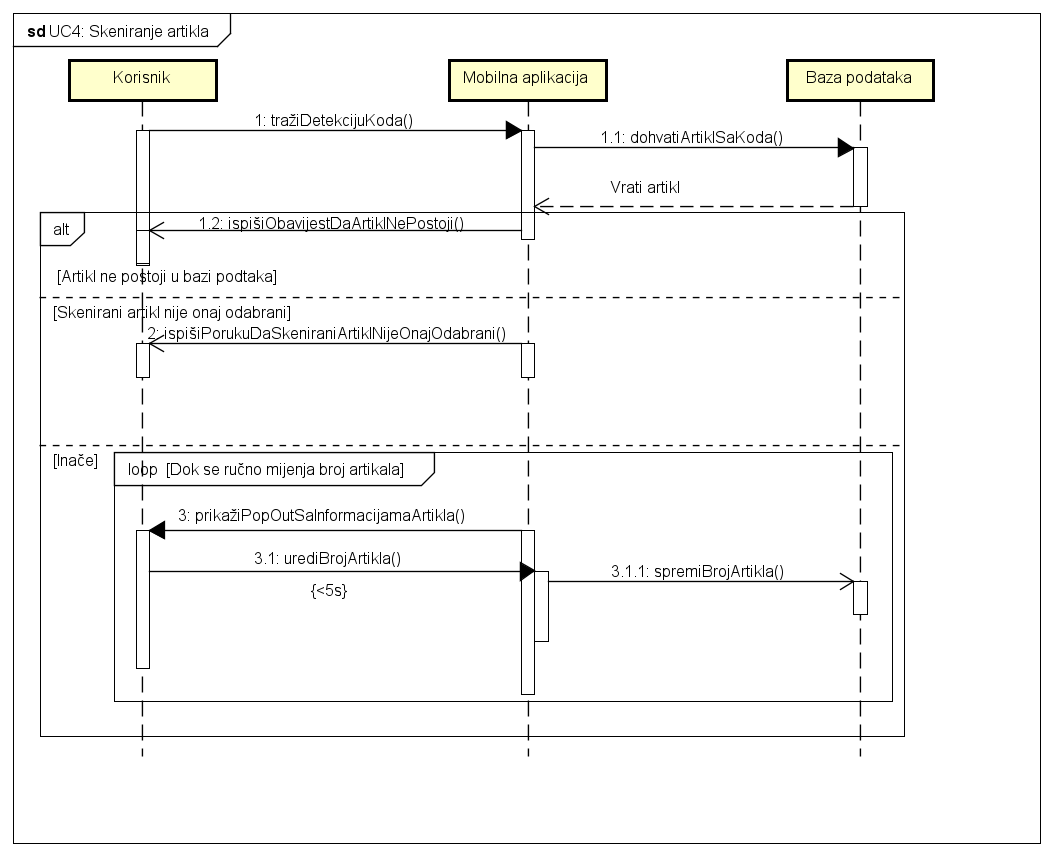
\includegraphics[scale=0.5]{slike/sekUC4.png}
				\caption{Sekvencijski dijagram za UC4}
			\end{figure}
				
			\textbf{Obrazac uporabe UC16 - Preraspodjela artikla}
			
			Korisnik šalje zahtjev mobilnoj aplikaciji za prikazom stabla proizvoda. Mobilna aplikacija dohvaća stablo proizvoda i prikazuje ga korisniku. Korisnik dok ne dođe do željenog proizvoda šalje zahtjeve za prikaz djece odabranog čvora. Kada korisnik odabere željeni list stabla mobilna aplikacija iz baze podataka dohvaća sve čvorove razine iznad izabranog lista. Mobilna aplikacija prikazuje sve čvorove razine iznad izabranog lista. Korisnik odabire novog roditelja. Nova struktura stabla se pohranjuje u bazu podataka.
			
			\begin{figure}[H]
				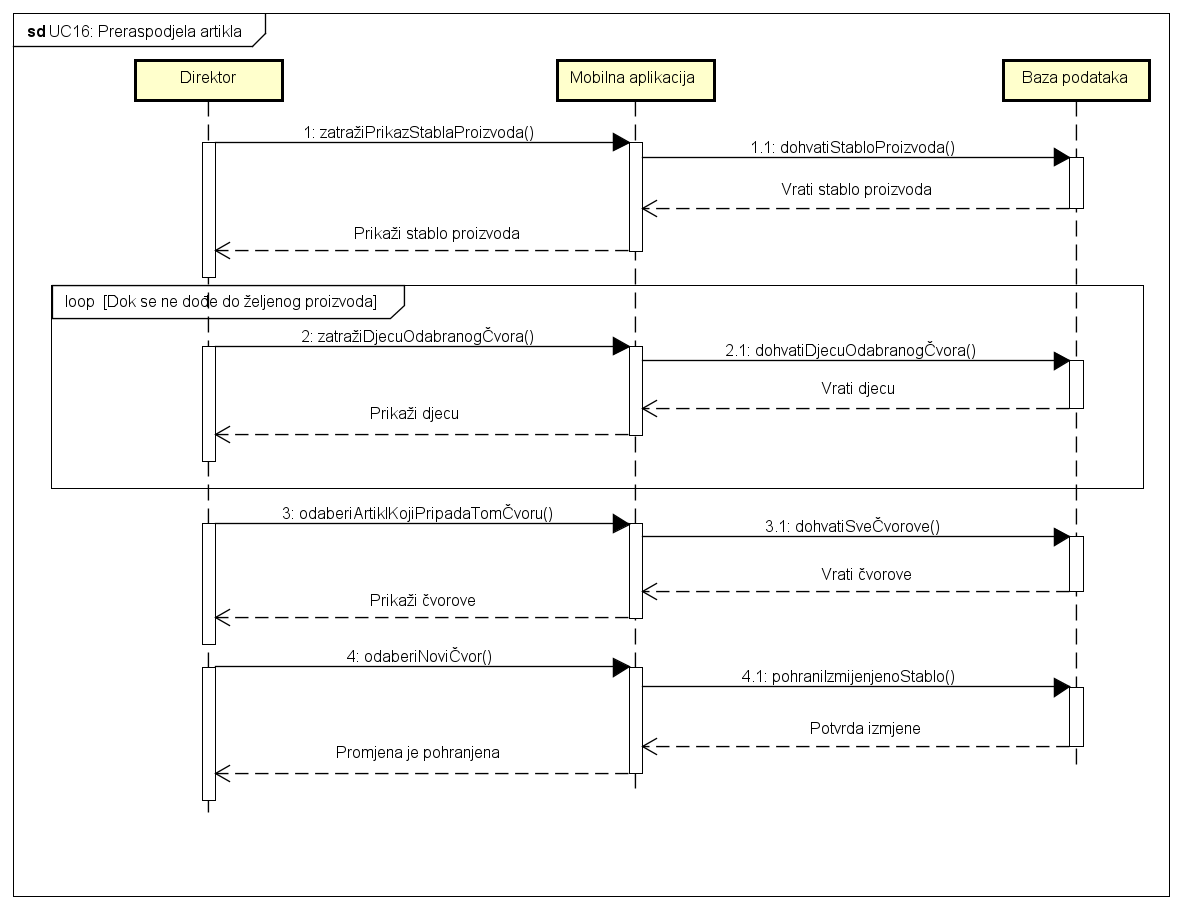
\includegraphics[scale=0.5]{slike/sekUC16.png}
				\caption{Sekvencijski dijagram za UC16}
			\end{figure}
		
			\textbf{Sekvencijski dijagram - završetak trenutne inventure}
			
			Korisnik od aplikacije traži završetak inventure. Aplikacija se povezuje s bazom podataka te od nje traži završetak trenutne inventure. U slučaju pogreške, to se dojavljuje korisniku pomoću pop-up prikaza. Ako je trenutna inventura uspješno završena, baza podataka to dojavljuje aplikacija, a ona dalje korisniku. Aplikacija nakon toga implicitno pokreće novu inventuru. Ukoliko se prilikom stvaranja nove inventure dogodi pogreška, status pogreške se dojavljuje korisniku.
			
			\begin{figure}[H]
				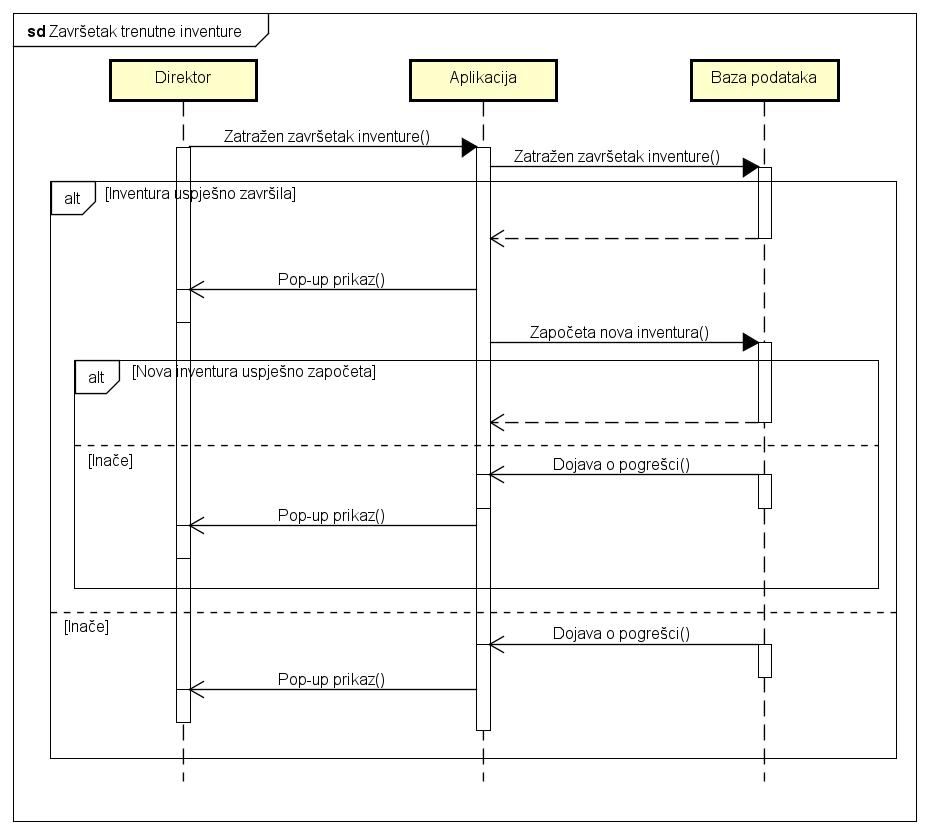
\includegraphics[scale=0.5]{slike/Sekvencijski dijagram.jpg}
				\caption{Sekvencijski dijagram za završetak trenutne inventure}
			\end{figure}
	
		\section{Ostali zahtjevi}
		
			\begin{packed_item}
				\item Sustav treba omogućiti rad više korisnika u stvarnom vremenu
				\item Korisničko sučelje i sustav moraju podržavati hrvatsku abecedu (dijakritičke znakove) pri unosu i prikazu tekstualnog sadržaja
				\item Sustav treba dohvaćati lokaciju korisnika preko GPS modula
				\item Izvršavanje dijela programa u kojem se pristupa bazi podataka ne smije trajati duže od nekoliko sekundi 
				\item Sustav treba biti implementiran kao mobilna aplikacija koristeći objektno-orijentirane jezike

				\item Neispravno korištenje korisničkog sučelja ne smije narušiti funkcionalnost i rad sustava

				\item Sustav treba biti jednostavan za korištenje, korisnici se moraju znati koristiti sučeljem bez opširnih uputa 
				\item Veza s bazom podataka mora biti kvalitetno zaštićena, brza i otporna na vanjske greške
			\end{packed_item}
			 
			 
			 
	